\chapter{Layered Entrepreneurial Leverage in San Antonio}

This lecture gives us no blackboard to copy, but it does give us a precise order of ideas. We are first shown scale, then warned about the danger of reckless scaling, then reminded that personal stability and daily conduct are themselves productive forces, and only after that are we led through land, craft, short-term rentals, and exotic cars. To keep the quantitative claims legible, we introduce a light bookkeeping notation for gross revenue, net worth, and time scale, while staying close to the way the speaker unfolds the subject.

\section{Opening Benchmarks: Wealth Before Method}

The lecture begins with outcomes before mechanisms. A teaser around the R8, followed by quick questions about the largest amount made in a single year, sets the stakes first. We are meant to feel the scale before we are told how the scale was produced.

\begin{definition}
We write \(G\) for gross revenue or income, \(NW\) for net worth, and use subscripts \(y\), \(m\), and \(d\) for yearly, monthly, and daily time scales. This is bookkeeping notation for the notes, not notation spoken in the lecture.
\end{definition}

The opening numbers are therefore best read as scale markers:
\begin{align}
G_{y,\max}
&\in
\{\$1{,}000{,}000,\;>\$500{,}000,\;\$300{,}000\text{--}\$400{,}000,\;\$1.3\times 10^6\ \text{gross}\},\\
NW
&\approx \$15\text{M}\text{--}\$20\text{M}.
\end{align}

What matters about this opening is not merely the size of the numbers. It is the order in which they appear. The lecture refuses to begin with theory. First we see the endpoint; then we ask which operating rules, capital choices, and habits can plausibly generate it.

\section{Scaling Without Self-Destruction}

\paragraph{Anecdote.}
The first substantial respondent has worked across several roles---wealth management, corporate leadership, and construction. The interviewer asks what was implemented in order to scale businesses.

\paragraph{Claim.}
The answer is a control law for growth: we do not jump straight to maximum size. We move in stages.

\begin{equation}
\text{crawl} \longrightarrow \text{walk} \longrightarrow \text{run}.
\end{equation}

\paragraph{Mechanism.}
The point is not merely motivational pacing. It is a relation between learning speed and leverage speed. If debt and obligations grow faster than competence, then a setback arrives before recovery capacity has been built. The speaker's warning is therefore structural: over-leverage is what happens when scale outruns understanding.

\subsection{Question \& Answer}

\paragraph{Question.}
How do we scale without breaking the business?

\paragraph{Answer.}
The lecture's answer is to constrain the step size. We first build a model that can survive small errors, then a model that can survive medium errors, and only then a model that can tolerate aggressive expansion. In entrepreneurial language, this means expertise before acceleration and resilience before debt. The point is not to avoid growth. The point is to grow in a way that preserves the ability to stand back up.

From here the lecture makes a sharp and important turn. Scale alone is not enough. We are now told that the condition for sustained business success includes personal structure and reputation.

\section{Personal Stability, Daily Conduct, and Entrepreneurial Endurance}

\paragraph{Anecdote.}
When asked about the best financial decision of his career, the same respondent answers by pointing to marriage. Immediately after that, the advice to a younger self becomes: every day is an interview; every day is your resume.

\paragraph{Claim.}
This is a strong claim about economic life. The lecture is telling us that business success is not exhausted by transactions, balance sheets, and formal interviews. Character, attitude, and ordinary daily conduct are part of the production process.

\paragraph{Mechanism.}
If opportunities are allocated through trust, referrals, hiring decisions, partnerships, and repeated contact, then reputation accumulates through daily behavior. The transcript does not turn this into formal notation, and we should not force one. But the logic is cumulative: repeated conduct shapes the set of opportunities one is later offered.

The caricature intermission then resets the pace, and a new entrepreneur appears: a founder from bioinformatics, combining computer science and medical training, who has already sold a business. The focus changes from life structure to endurance under pressure.

\subsection{Question \& Answer}

\paragraph{Question.}
What matters most when a business looks as if it may fail?

\paragraph{Answer.}
The lecture answers with perseverance. The founder's view is that friction is not an exception to growth but one of its conditions. If adversity is guaranteed, then the operative variable is not whether friction appears, but whether the entrepreneur remains in motion long enough to learn from it.

The section ends with a forward-looking pivot to AI. The speaker does not present AI as magical replacement. The sharper claim is that the relevant competitive edge lies with the person who knows how to use AI well. In other words, the lecture shifts from raw technology to complementarity with technology.

\section{Capital Allocation, Scarcity, Craft, and Lifestyle Choice}

The hotel sequence moves the lecture from earnings to capital placement. Once people start making money, where should that money go if it is to multiply rather than merely be spent?

\paragraph{Anecdote.}
A real-estate developer recommends land. The justification is concrete: the supply is fixed, development costs rise, land can later be developed, and agricultural use may lower the current tax burden.

\paragraph{Claim.}
The lecture's capital-allocation claim is that scarce, re-usable assets can amplify earnings if they are chosen with patience.

\paragraph{Mechanism.}
A compact way to summarize the developer's logic is
\begin{equation}
\dot S_{\mathrm{land}} \approx 0,
\qquad
\dot C_{\mathrm{develop}} > 0.
\end{equation}
This is editorial shorthand, not spoken notation. Its meaning is simple: supply is effectively fixed while development costs tend to rise. Under that combination, the option value of land can be substantial, especially if current carrying costs are moderated by favorable tax treatment.

\subsection{Question \& Answer}

\paragraph{Question.}
Where should earned money go if we want it to multiply?

\paragraph{Answer.}
One answer offered by the lecture is land: scarce supply, future development optionality, and a path from present holding to later capital gains. But the lecture does not stop there, and that is crucial. It immediately widens the evidence.

We next meet a caricature artist with roughly \(35\) years in the craft, a stated peak annual income in the \(\$300{,}000\text{--}\$400{,}000\) range, and a claim to have drawn almost half a million people. Then we meet an architect who owns a solo practice. These interviews prevent us from treating scalable asset businesses as the only path.

For the caricature artist, one can at least record the scale marker
\begin{equation}
G_{y,\max}^{\mathrm{artist}} \approx \$300{,}000\text{--}\$400{,}000.
\end{equation}
The point, however, is larger than the number. Long repetition, highly visible craft, and refusal to quit can also generate major earnings. The architect extends the point in a different direction: career choice is constrained by the lifestyle one wants. The lecture thereby adds another hidden variable to our model of entrepreneurship, namely that income must be read together with the form of life that produces it.

By the end of this stretch, the lecture has given us three distinct mechanisms: scarcity in land, endurance in craft, and self-direction in professional practice. Only after this does it return to the R8 owner and begin the most explicit case study in repeatable enterprise.

\section{From the First Property to a Repeatable Portfolio}

\paragraph{Anecdote.}
The R8 owner says that real estate was the first major investment. He reports a gross total of about \(\$1.3\) million in a single year and says that the combined total of units and properties is about \(38\text{--}40\).

\paragraph{Claim.}
The lecture's main operational claim now comes into focus: begin with something one is willing to learn deeply, then duplicate what works. Passion is not treated as sentiment; it is treated as a fuel for sustained attention. Humility then appears as the control variable that keeps learning open.

\paragraph{Mechanism.}
The speaker's own description has a clear order: become interested, invest effort, learn the system around the thing, and then repeat the same deal structure. This is the lecture's transition from isolated success to an actual operating model.

We therefore record the main portfolio data as
\begin{equation}
N_{\mathrm{holdings}} \approx 38\text{--}40,
\qquad
G_{\mathrm{portfolio},y} \approx \$1.3\times 10^6 \ \text{gross}.
\end{equation}

\subsection{Question \& Answer}

\paragraph{Question.}
If we had zero properties and zero rentals, what is the first move toward the first deal?

\paragraph{Answer.}
The lecture answers with research, and the answer is more concrete than it sounds. Research here means: examine the city, examine the area, examine the platform, and study what is already working in that market. Only then do we choose an offering and enter.

A compact transcript-derived schematic is helpful:

\begin{figure}[t]
\centering
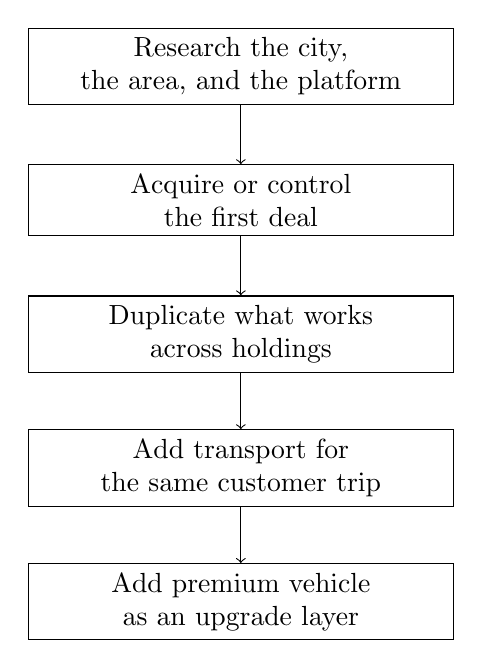
\begin{tikzpicture}[x=1cm,y=1cm]
\node[draw,align=center,minimum width=5.4cm,minimum height=0.9cm] (a) at (0,0) {Research the city,\\the area, and the platform};
\node[draw,align=center,minimum width=5.4cm,minimum height=0.9cm] (b) at (0,-1.7) {Acquire or control\\the first deal};
\node[draw,align=center,minimum width=5.4cm,minimum height=0.9cm] (c) at (0,-3.4) {Duplicate what works\\across holdings};
\node[draw,align=center,minimum width=5.4cm,minimum height=0.9cm] (d) at (0,-5.1) {Add transport for\\the same customer trip};
\node[draw,align=center,minimum width=5.4cm,minimum height=0.9cm] (e) at (0,-6.8) {Add premium vehicle\\as an upgrade layer};
\draw[->] (a) -- (b);
\draw[->] (b) -- (c);
\draw[->] (c) -- (d);
\draw[->] (d) -- (e);
\end{tikzpicture}
\caption{A transcript-derived ladder of leverage. The lecture moves from research, to a first property, to duplication, and finally to adjacent revenue layers built around the same trip.}
\end{figure}

At this point the lecture gives us numbers that support a worked example. The speaker says that one property can gross roughly \(\$3{,}000\text{--}\$5{,}500\) per month. If we annualize that range, we obtain
\begin{align}
G_{\mathrm{property},y}
&= 12\,G_{\mathrm{property},m} \\
&\approx 12\times (\$3{,}000\text{--}\$5{,}500) \\
&\approx \$36{,}000\text{--}\$66{,}000.
\end{align}

We can also perform a rough portfolio-average calculation:
\begin{align}
\bar G_{\mathrm{holding},y}
&= \frac{G_{\mathrm{portfolio},y}}{N_{\mathrm{holdings}}} \\
&\approx \frac{\$1.3\times 10^6}{38\text{--}40} \\
&\approx \$32{,}500\text{--}\$34{,}200.
\end{align}

The comparison is instructive. The implied portfolio-wide average per holding is lower than the upper end of the quoted single-property range. That is not a contradiction. The transcript itself tells us that the holding count mixes units and properties, and the \(\$1.3\) million figure is given as gross total. The point of the arithmetic is therefore not precision but scale: the lecture is showing us that a repeatable model, applied many times, can turn a moderate unit-level gross into a large annual total.

\section{Layered Enterprise: From Lodging to Transport to the R8}

The final and most operationally dense movement of the lecture begins with a simple observation: a customer who books a stay also has transportation needs. Once that is seen, a second business can be built on top of the first.

\paragraph{Anecdote.}
The R8 owner explains that the exotic car business came after the property business. Guests book a property, then need transport, and then may want a premium experience. Turo is described as an Airbnb-like platform for cars.

\paragraph{Claim.}
The lecture's most important enterprise claim is that adjacent services can be layered on the same demand event. We do not always need a new customer to start a new line of business. Sometimes we need to understand the full chain of needs created by the customer we already have.

\paragraph{Mechanism.}
A clean bookkeeping identity for this last move is
\begin{equation}
R_{\mathrm{trip}}
=
R_{\mathrm{lodging}}
+
R_{\mathrm{transport}}
+
R_{\mathrm{premium}}.
\end{equation}
This is not a quoted formula from the speaker; it is the simplest way to preserve the logic of the interview. A single trip can generate lodging revenue, regular transport revenue, and then premium-upgrade revenue.

The lecture then supplies the sharpest operating numbers in the chapter. Some cars, we are told, can make about \(\$8{,}000\text{--}\$10{,}000\) per month, while the R8 typically rents for about \(\$600\text{--}\$700\) per day, depending on booking length. We therefore write
\begin{equation}
G_{R8,m}=p_{R8,d}\,d_{R8,m},
\qquad
p_{R8,d}\approx \$600\text{--}\$700.
\end{equation}

Now we can do a cautious consistency check. If we use the monthly figure only as an order-of-magnitude benchmark for a premium car, then the implied booked days per month satisfy
\begin{align}
d_{R8,m}
&= \frac{G_{R8,m}}{p_{R8,d}} \\
&\approx
\frac{\$8{,}000\text{--}\$10{,}000}{\$700\text{--}\$600} \\
&\approx 11.4\text{--}16.7 \ \text{booked days per month}.
\end{align}

This should be read carefully. The interview says that \(\$8{,}000\text{--}\$10{,}000\) can occur on some cars, not necessarily that the R8 itself always realizes that figure. Still, the arithmetic shows why the business is plausible: at a daily rate of roughly \(\$600\text{--}\$700\), consistent weekend demand already points toward meaningful monthly gross.

\subsection{Question \& Answer}

\paragraph{Question.}
How do we add a second revenue layer without starting from scratch?

\paragraph{Answer.}
The lecture's answer is not to chase random diversification. We add the second layer by following the first customer's next need. Property guests need transportation; some transportation demand can be served by ordinary cars; some can be served by premium vehicles. The enterprise grows not by abandoning the first business but by standing on it.

The last question in the lecture---how to begin in the exotic car rental business---returns us to the earlier theme of controlled scale. Form the LLC, learn how to place vehicles inside it, build business credit when necessary, and do not forget that this layer works best when it sits on top of something else already functioning.

\section{Summary}

The lecture begins with spectacle and ends with structure. We are first shown million-dollar years and an Audi R8, but the deeper content lies elsewhere: scale must be staged; debt must not outrun competence; reputation accumulates daily; perseverance matters when friction appears; land derives value from scarcity and future optionality; craft and self-owned practice remain valid paths; research precedes the first deal; duplication creates portfolio scale; and the strongest businesses often add layers around the same customer rather than hunting endlessly for unrelated revenue.

What we finally obtain is a compact entrepreneurship model. The first layer is discipline and judgment. The second layer is a repeatable asset or operating system. The third layer is adjacent monetization. In the language of the lecture, we do not simply get rich by moving faster. We get rich by learning what to repeat, what to own, and what can be added on top.